% CS 418: Intro to Data Science — Worksheet 17 (17-week09-day1)
% Week 9, Monday 2026-10-19

% Compile with: latexmk -pdf worksheet.tex

\documentclass[11pt]{article}

% ── Packages ──────────────────────────────────────────────────────────────────
\usepackage[margin=0.65in, headheight=14pt]{geometry}
\usepackage{amsmath, amssymb}
\usepackage{ragged2e}
% Never break a word across lines, including at hyphens ("Sans-Serif").
\hyphenpenalty=10000
\exhyphenpenalty=10000
\usepackage{enumitem}
\usepackage{booktabs}
\usepackage{graphicx}
\usepackage{hyperref}
\usepackage{xcolor}
\usepackage{fancyhdr}
\usepackage{mdframed}
\usepackage{array}
\usepackage{tikz}

% ── Page style ────────────────────────────────────────────────────────────────
\pagestyle{fancy}
\fancyhf{}
\lhead{\textbf{CS 418: Intro to Data Science}}
\rhead{UIC, Fall 2026}
\cfoot{\thepage}
\renewcommand{\headrulewidth}{1pt}
\setlength{\headheight}{12pt}
\setlength{\headsep}{0.4cm}

% ── Hyperlinks ────────────────────────────────────────────────────────────────
\hypersetup{colorlinks=false, hidelinks}

% ── Convenience environments ──────────────────────────────────────────────────
% Usage: \blankspace{6cm} — blank area for hand-written work, no rules
\newcommand{\blankspace}[1]{%
  \vspace{0.3em}
  \begin{minipage}[t][#1][t]{\linewidth}
  \end{minipage}
  \vspace{0.3em}
}

% Usage: \guidedopen{title}{guided content}{guided workspace height}{open-ended workspace height}
% Left: a titled, structured prompt with its own blank workspace. Right: a fully blank workspace for open-ended exploration of the same topic (no prompt text), sized so the two columns land at roughly the same total height. Neither workspace is ruled.
\newcommand{\guidedopen}[4]{%
  \noindent\textbf{#1}\\[0.18em]
  \noindent
  \begin{minipage}[t]{0.485\textwidth}
    #2
    \blankspace{#3}
  \end{minipage}
  \hfill
  \begin{minipage}[t]{0.485\textwidth}
    \blankspace{#4}
  \end{minipage}
  \\[0.4em]
}

% Usage: \panelbox{width}{height}{caption} — a framed drawing panel with `caption` centered beneath it. An empty caption leaves the panel bare, with nothing below the frame at all.
\newcommand{\panelbox}[3]{%
  \begin{minipage}[t]{\dimexpr#1+2\fboxsep+2\fboxrule\relax}
    \framebox[#1][c]{\rule{0pt}{#2}}%
    \if\relax\detokenize{#3}\relax\else
      \\[0.25em]{\centering\small #3\par}%
    \fi
  \end{minipage}%
}

% Usage: \courserow{course} — one row of the neighbor survey: a course, then six empty cells (self and five neighbors).
\newcommand{\courserow}[1]{\small #1 & \rule{0pt}{0.36cm} & & & & & \\ \hline}

% Usage: \simrow{label} — one row of the binary similarity table: a neighbor, then six empty cells.
\newcommand{\simrow}[1]{\small #1 & \rule{0pt}{0.4cm} & & & & & \\ \hline}

% Usage: \splitsketch — the slides' 30 students (20 pass, 10 fail) as a parent node and two children with blank counts.
\newcommand{\splitsketch}{%
  \begin{tikzpicture}[box/.style={draw, minimum height=0.8cm, inner sep=4pt}]
    \node[box] (p) at (0,0) {20 pass, 10 fail};
    \node[box] (n) at (-2.3,-2.4) {\underline{\hspace{0.8cm}} pass, \underline{\hspace{0.8cm}} fail};
    \node[box] (y) at (2.3,-2.4) {\underline{\hspace{0.8cm}} pass, \underline{\hspace{0.8cm}} fail};
    \draw (p.south) -- node[above left, font=\small] {no} (n.north);
    \draw (p.south) -- node[above right, font=\small] {yes} (y.north);
  \end{tikzpicture}%
}

% Checkpoints 5, 6, and 7 each sit in a full-width block of this exact height, so they get the same space.
\newlength{\cpheight}
\setlength{\cpheight}{5.7cm}

% Usage: \fixedblock{content} — a full-width block exactly \cpheight tall.
\newcommand{\fixedblock}[1]{\noindent\begin{minipage}[t][\cpheight][t]{\linewidth}#1\end{minipage}\par}

% ══════════════════════════════════════════════════════════════════════════════
\begin{document}
\RaggedRight

% ── Title block: topic left, info box right ───────────────────────────────────
\noindent
\begin{minipage}[t]{0.55\textwidth}
  \vspace{0pt}
  {\LARGE \textbf{Worksheet \#\,17}} \\[0.18em]
  {\large \textit{Week 9, Day 1: k-NN and decision trees}}
\end{minipage}
\hfill
\begin{minipage}[t]{0.40\textwidth}
  \vspace{0pt}
  \small
  Name: \underline{\hspace{4.5cm}} \\[0.35em]
  NetID: \underline{\hspace{4.3cm}} \\[0.35em]
  Date: \underline{\hspace{4.4cm}} \\
\end{minipage}

\vspace{0.6em}
\noindent\rule{\linewidth}{0.6pt}
\vspace{0.1em}

\noindent\underline{\textbf{Guided checkpoints}}\\[0.2em]
\noindent{\small For full credit, fill in the checkpoints. If you skip a checkpoint, you must include your own notes for full credit.}
\vspace{0.8em}

% ── 1. Neighbor survey ───────────────────────────────────────────────────────
% Rows: four BS CS required courses, four technical electives, four others (titles from catalog.uic.edu, Oct. 2026).
\noindent\textbf{1. Talk to Your Neighbors}\\[0.18em]
\noindent Fill in the Self column for yourself. Then talk to five classmates (at most one of them can be in your project group) and fill in each cell with 1 if they have taken the course or 0 if they have not.

\vspace{0.5em}

\noindent
{\setlength{\tabcolsep}{4pt}%
\begin{tabular}{|l|*{6}{>{\centering\arraybackslash}p{1.45cm}|}}
  \hline
  \small Course & \scriptsize Self & \scriptsize Neighbor 1 & \scriptsize Neighbor 2 & \scriptsize Neighbor 3 & \scriptsize Neighbor 4 & \scriptsize Neighbor 5 \\
  \small Name: & \rule{0pt}{0.55cm} & & & & & \\ \hline\hline
  \courserow{CS 100 Discovering Computer Science}
  \courserow{CS 251 Data Structures}
  \courserow{CS 301 Languages and Automata}
  \courserow{CS 361 Systems Programming}
  \courserow{CS 401 Computer Algorithms I}
  \courserow{CS 411 Artificial Intelligence I}
  \courserow{CS 412 Introduction to Machine Learning}
  \courserow{CS 424 Visualization and Visual Analytics}
  \courserow{CS 426 Video Game Design and Development}
  \courserow{CS 427 Creative Coding}
  \courserow{CS 480 Database Systems}
  \courserow{CS 488 Introduction to Cryptography}
\end{tabular}}

\vspace{0.5em}

\vfill

% ── 2. Binary similarity ─────────────────────────────────────────────────────
\noindent
\begin{minipage}{\linewidth}
\noindent\textbf{2. Binary Similarity}\\[0.18em]
\noindent Compare your Self column with each neighbor from checkpoint 1. Count $N_{11}$ (both took it), $N_{10}$ (only you), $N_{01}$ (only your neighbor), and $N_{00}$ (neither), then compute Jaccard and SMC.

\vspace{0.5em}

\noindent
\begin{tabular}{|l|*{6}{>{\centering\arraybackslash}p{1.9cm}|}}
  \hline
  & \small $N_{11}$ & \small $N_{10}$ & \small $N_{01}$ & \small $N_{00}$ & \small Jaccard & \small SMC \\ \hline
  \simrow{Neighbor 1}
  \simrow{Neighbor 2}
  \simrow{Neighbor 3}
  \simrow{Neighbor 4}
  \simrow{Neighbor 5}
\end{tabular}

\vspace{0.6em}
\noindent Nearest neighbor by Jaccard: \underline{\hspace{3.5cm}} \hfill Nearest neighbor by SMC: \underline{\hspace{3.5cm}}
\end{minipage}

\vspace{0.6em}

\vfill

% ── 3. Jaccard vs. SMC ───────────────────────────────────────────────────────
\guidedopen{3. Jaccard vs. SMC}{
\raggedright What is the difference between Jaccard and SMC?
}{1.6cm}{3.4cm}

\vfill

\newpage

% ── 4. Distance metrics ──────────────────────────────────────────────────────
\guidedopen{4. Distance Metrics}{
\raggedright Plot two points, then draw and label the Euclidean and Manhattan paths.

\vspace{0.5em}
\noindent
\begin{minipage}[c]{0.62\linewidth}
\begin{tikzpicture}[scale=0.8]
  \draw[step=1, gray!50, thin] (0,0) grid (5,5);
  \draw[->] (0,0) -- (5.4,0);
  \draw[->] (0,0) -- (0,5.4);
  \foreach \i in {0,...,5} {
    \node[below, font=\scriptsize] at (\i,0) {\i};
    \node[left, font=\scriptsize] at (0,\i) {\i};
  }
\end{tikzpicture}
\end{minipage}%
\begin{minipage}[c]{0.38\linewidth}
Euclidean:
\vspace{1.6cm}

Manhattan:
\vspace{0.6cm}
\end{minipage}
}{0.1cm}{5.4cm}

\vfill

% ── 5. Memorizing vs. generalizing ──────────────────────────────────────────
\fixedblock{\guidedopen{5. Memorizing vs. Generalizing}{
\raggedright In your own words, what is the difference between memorizing and generalizing?
}{0.1cm}{0.1cm}}

\vfill

% ── 6. Good split, bad split ─────────────────────────────────────────────────
\fixedblock{%
\noindent\textbf{6. Good Split, Bad Split}\\[0.18em]
\noindent
\begin{minipage}[t]{0.485\linewidth}
\noindent Good split:\\[0.2em]
\splitsketch
\end{minipage}
\hfill
\begin{minipage}[t]{0.485\linewidth}
\noindent Bad split:\\[0.2em]
\splitsketch
\end{minipage}}

\vfill

% ── 7. Information gain ──────────────────────────────────────────────────────
\fixedblock{\guidedopen{7. How Much Does a Split Help?}{
\raggedright What metric(s) can be used to determine how much a split helps distinguish classes?
}{0.1cm}{0.1cm}}

\vfill

\end{document}
